\chapter{Aufgabe 1}

\lstset{language=Java,
	showspaces=false,
	showtabs=false,
	breaklines=true,
	showstringspaces=false,
	breakatwhitespace=true,
}


\definecolor{dkgreen}{rgb}{0,0.6,0}
\definecolor{gray}{rgb}{0.5,0.5,0.5}
\definecolor{mauve}{rgb}{0.58,0,0.82}

\lstset{	
	frame=tb,
	language=Java,
	aboveskip=3mm,
	belowskip=3mm,
	showstringspaces=false,
	columns=flexible,
	basicstyle={\small\ttfamily},
	numbers=none,
	numberstyle=\tiny\color{gray},
	keywordstyle=\color{blue},
	commentstyle=\color{dkgreen},
	stringstyle=\color{mauve},
	breaklines=true,
	breakatwhitespace=true,
	tabsize=3,
	backgroundcolor=\color{black!5},
	numbers=left, stepnumber=1, numberstyle = \tiny
	% set backgroundcolor
}

\section{a}
\begin{figure}[h!]
	\centering
	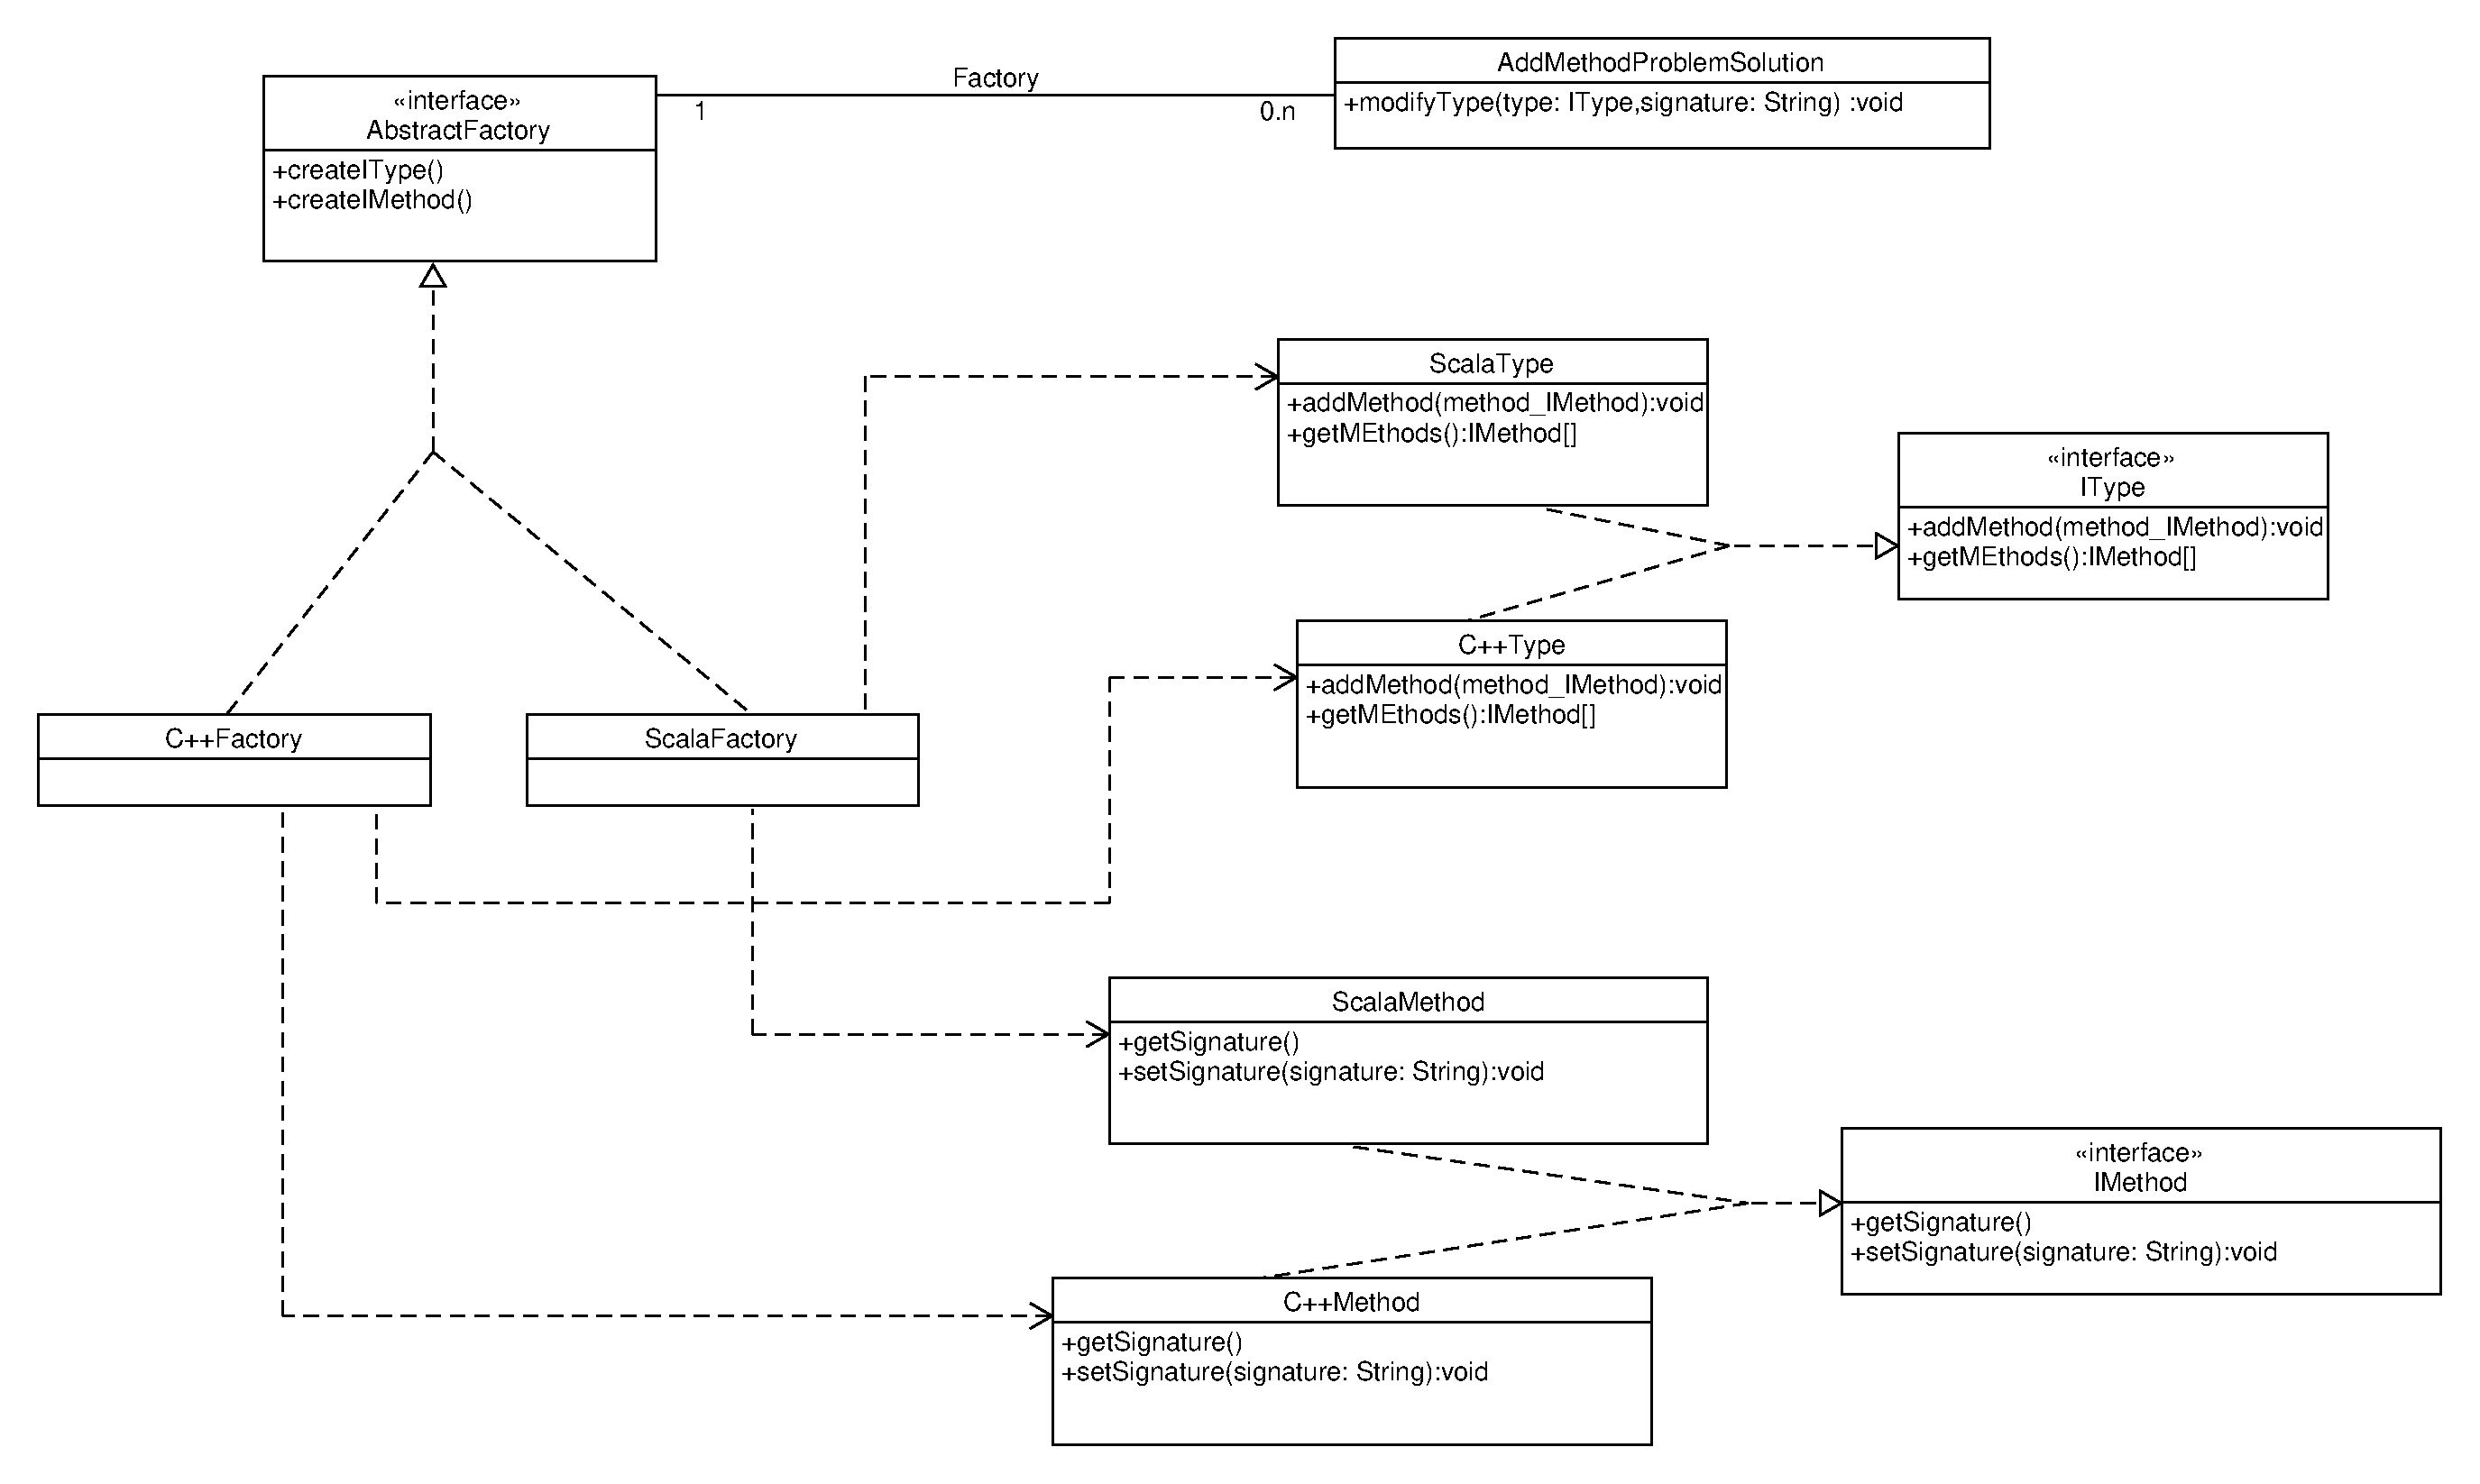
\includegraphics[width=0.8\textwidth, clip]{images/AbstractFactoryMyIDE_UML.pdf}
	\caption{UML Diagramm von MyIDE mit  AbstractFactory Pattern.}
	\label{fig:ULM}
\end{figure}
\section{b}


\begin{lstlisting}[ caption = {Aufgabe 1 b}]
	public ScalaMethod createIMethod(){  //retruntype evtl IMethod
		retrun new ScalaMethod();
	}
\end{lstlisting}


\section{c}
\begin{lstlisting}[caption = {Aufgabe 1 c}]
public void modifyType(IType type, String signature){
 	IMethod newMethod = factory.createIMethod();
 	newMethod.setSignature(signature);
	type.addMethod(newMethod);
}
\end{lstlisting}

\section{d}
Abstrakte Produkte:\\
IType, IMethod\\


Konkrete Implemntierung der abstrakten Fabrik:\\
ScalaFactory, C++Factory\\


Konkrete Implementierung der Produkte:\\
ScalaType, C++Type, ScalaMethod, C++Method\\


Methoden zum Erstellen von Produkten:\\
createIType, createIMethod\\


Abstrakte Fabrik:\\
AbstractFactory\\




%
%\begin{lstlisting}[	caption = {Klasse Book}]
%package org.library;
%
%
%public String getAuthor() { return author; }
%
%// implementiert interface LibraryItem
%@Override
%public String getCatalogDescription() {
%return title + " by " + author;  
%}
%}
%\end{lstlisting}


